\chapter{Konzept}

\section{Neue Architektur}
Die neue Architektur soll eine gute und stabile Basis für alle drei Anwendungen bieten. Das soll durch das Erstellen von modularen Komponenten geschehen. 

Der Kernstruktur der drei Anwendungen soll identisch sein, sodass mit möglichst wenig unterschiedlichem Code notwendig ist um die verschiedenen 
Anwendungen zu erstellen. Bei den Softwaremodulen ist es wichtig, dass diese eine eindeutige Funktion haben, dass eindeutige Schnittstelen definiert sind
 und dass diese gut wiederverwendet werden können. 

\input{content/Konzept/konzeptBenutzeroberfläche}
\subsection{SimulatorInstance}
Die SimulatorInstance unterscheidet sich bei jeder Anwendungsausprägung. Jedoch gibt es Komponenten, welche von mehreren der Anwendungen verwendet werden 
können. Im Folgenden wird die Grundstruktur SimulatorInstance beschrieben, welche Komponenten diese verwenden kann und wie letztendlich die 
unterschiedlichen Instancen aufgeteilt sind.

Eine Komponente, die jede Instance enthält, ist ein Datenmodell. Es wurde entschieden, dass das Modell des RadarSimulators mit einer kleinen Erweiterung,
 für alle drei Anwendungen genutzt wird. Dadurch kann nicht nur der Modell-Code wiederverwendet werden, sondern auch der Code zum Erstellen und Verwalten 
des Modells bleibt identisch.

Da es nun eine Komponente gibt, die jede Anwendungsausprägung verwendet, ist es sinnvoll eine Klasse zu erstellen, die das Modell verwaltet und auf der 
die weiteren Simulator Instanzen aufbauen. Diese Klasse heißt SimulatorCore.





\newpage
\section{Features}

\subsection{Single Target Tracking}
Um Single Target Tracking zu ermöglichen, benötigt die Anwendung eine Erweiterung um zwei Funktionen. Zum einen muss überprüft werden, ob sich ein Ziel 
im Suchbereich befindet, wenn dies zutrifft, soll nach jeder Bewegung des Ziels, das Audiogate auf dessen Position gesetzt werden. Des Weiteren muss sich 
die Beamline, je nach Zielverfolgung oder Zielsuche korrekt verhalten.

Während der STT Modus aktiviert ist, bewegt sich die Beamline innerhalb eines engen Sektors wiederholt über das Ziel. Wenn kein Ziel gefunden wird, sucht
die Beamline in einem größeren Bereich nach einem neuen Ziel. Der Sektor hat das Audiogate als Mittelpunkt und ändert seinen Bereich synchron zum 
Audiogate. Wenn ein Ziel verfolgt wird beträgt die Breite des Sektors 100 mils. Falls der Sensor ein Ziel zur Verfolgung sucht, beträgt die 
Bewegungsweite 300 mils. Diese Funktion wird im BeamlineTask implementiert, da dieser Zugriff auf das Audiogate und die Beamlineinformationen hat. Der 
BeamlineTask hat jedoch keinen Zugriff auf die Daten der Tracks. Deshalb weiß er nicht, ob ein Ziel verfolgt wird und kann kein Audiogate setzen. Damit 
der Beamlinetask weiß, ob ein Ziel verfolgt wird, wird ein Booleanflag, welches jederzeit abgefragt werden kann, im Model hinzugefügt.

Das Flag, sowie das Audiogate sollen vom Trackupdater gestetzt werden. Dieser hat alle Informationen der verfügbaren Tracks, die in der Simulation 
existieren und kann berechnen, ob das Ziel derzeitig von der Beamline erfasst wird. Der TrackUpdater hat die Methode schedule(), welche wiederholt nach 
einem bestimmten Zeitintervall aufgerufen wird. Diese Methode aktualisiert die Tracks und sendet Track Informationen an den Sensor. Diese Methode wird 
nun erweitert, um das STTFlag und das Audiogate zu setzen. Ein verfolgter Track wird im TrackUpdater gespeichert.

Zum Anfang der Methode wird überprüft, ob bereits ein Track verfolgt wird, falls dies nicht der Fall ist wird die Distanz vom Audiogate zu allen 
vorhandenen Tracks berechnet. Die Werte werden in einer Liste mit dem jeweiligen Track gespeichert, wenn sie innerhalb des STT-Sektors liegen. Die 
STT-Funktion ist so definiert, dass sie den nächsten Track zum Audiogate innerhalb des Sektors so lange verfolgt, bis dieser verschwindet oder man das 
Audiogate manuell ändert. Deshalb wird die Liste so sortiert, damit der Track mit dem geringsten Abstand zum Audiogate an erster Stelle steht. Nachdem 
sortiert wurde, wird das erste Element gespeichert, das Flag wird auf true gesetzt und die Liste wird geleert. Wenn die Liste leer ist wird nichts getan. 

Wird bereits ein Track verfolgt, wird geprüft, ob der zu verfolgende Track aktuell existiert. Das passiert indem man in der Liste, der gegenwärtigen 
Tracks nach einem Track mit der identischen ID des gespeicherten Tracks ist sucht. Ist dieser vorhanden, wird dieser Track als neuer Track gespeichert. 
Als nächstes wird getestet, ob dieser Track vom Sensor detektiert wird.  Trifft es zu, dass der Track vorhanden ist und detektiert wird setzt der 
TrackUpdater das Audiogate auf die aktuelle Position des Tracks. Wenn der Track nicht detektiert wird oder existiert, wird ein Zähler hochgezählt. Es 
kann passieren, dass ein Track in einem oder mehreren Durchläufen nicht im Bereich der Beamline liegt oder dass der Track vom Sensor nicht erfasst wird, 
da er z.B. zu weit entfernt ist. Durch den Zähler kann man einen Toleranzwert festlegen, wie oft der Track nicht erkannt werden muss bevor diesem nicht 
mehr gefolgt wird. Dem Track wird entfolgt, indem das Flag auf false gesetzt und der Track gelöscht wird.

\begin{figure}[h]
    \centering
    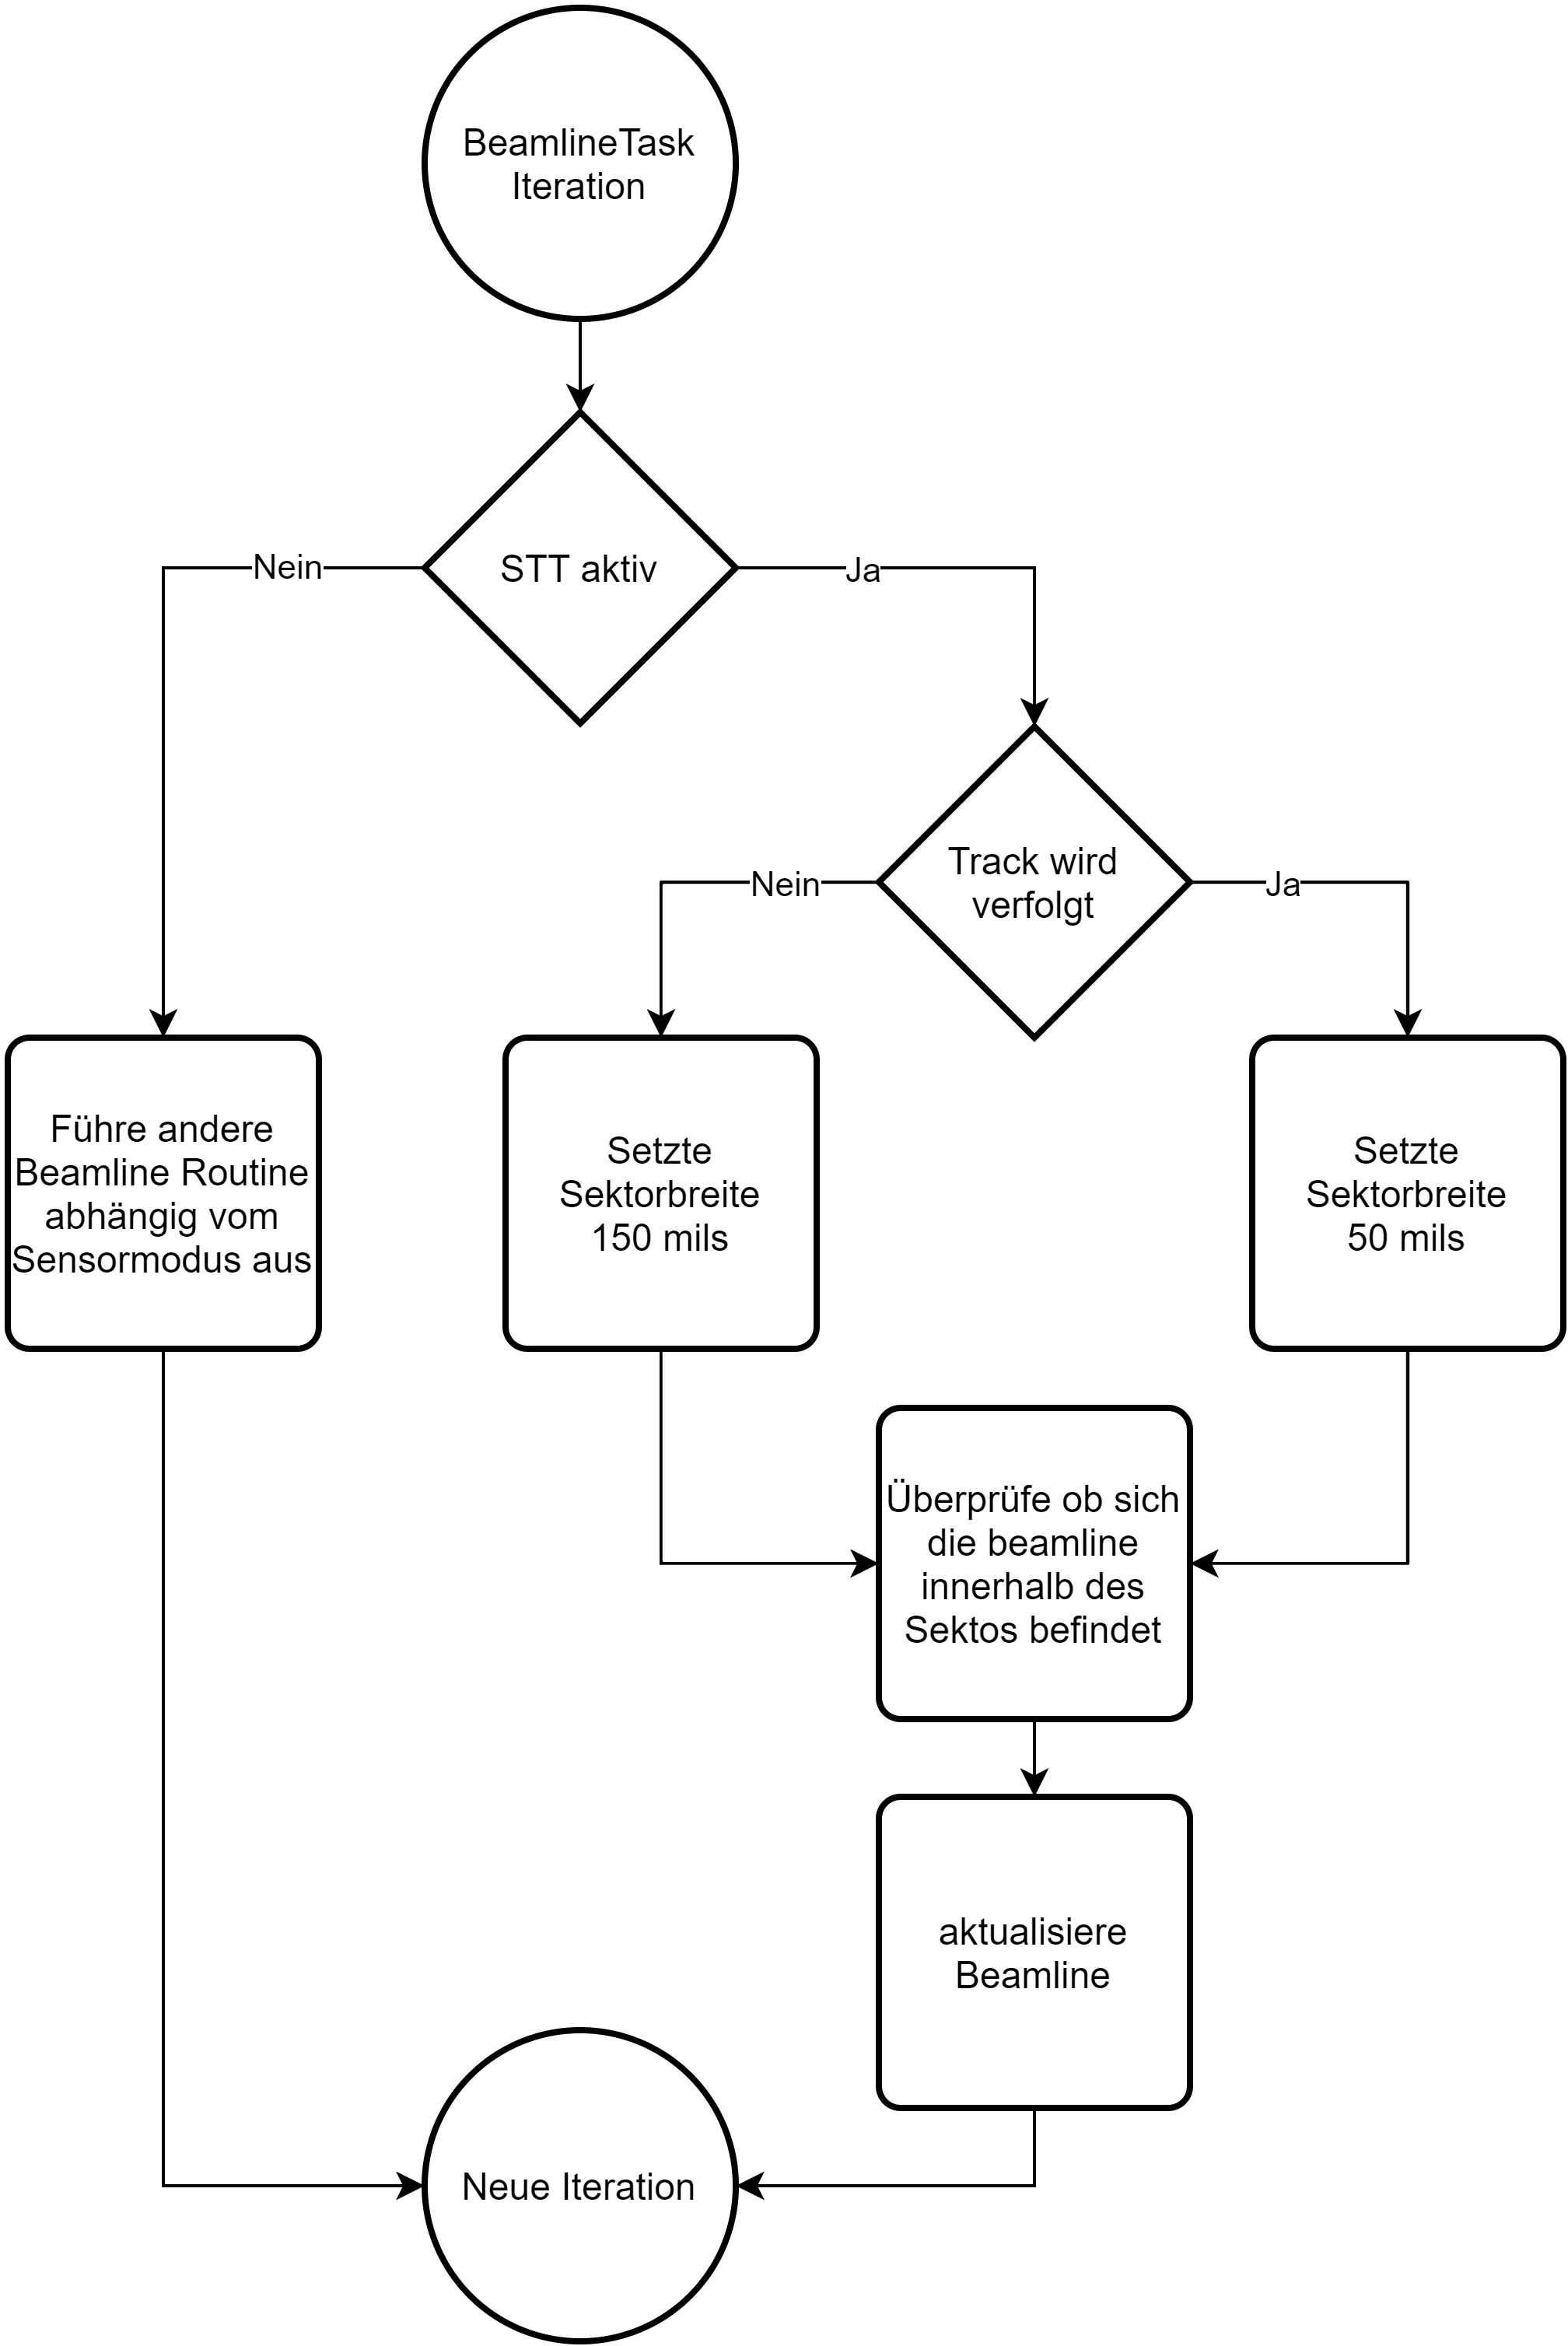
\includegraphics[width=0.6\textwidth]{content/assets/BeamlineTaskSTT.png}
    \caption{Flussdiagramm des Algorithmus des BeamlineTask}
\end{figure}

\begin{figure}[h]
    \centering
    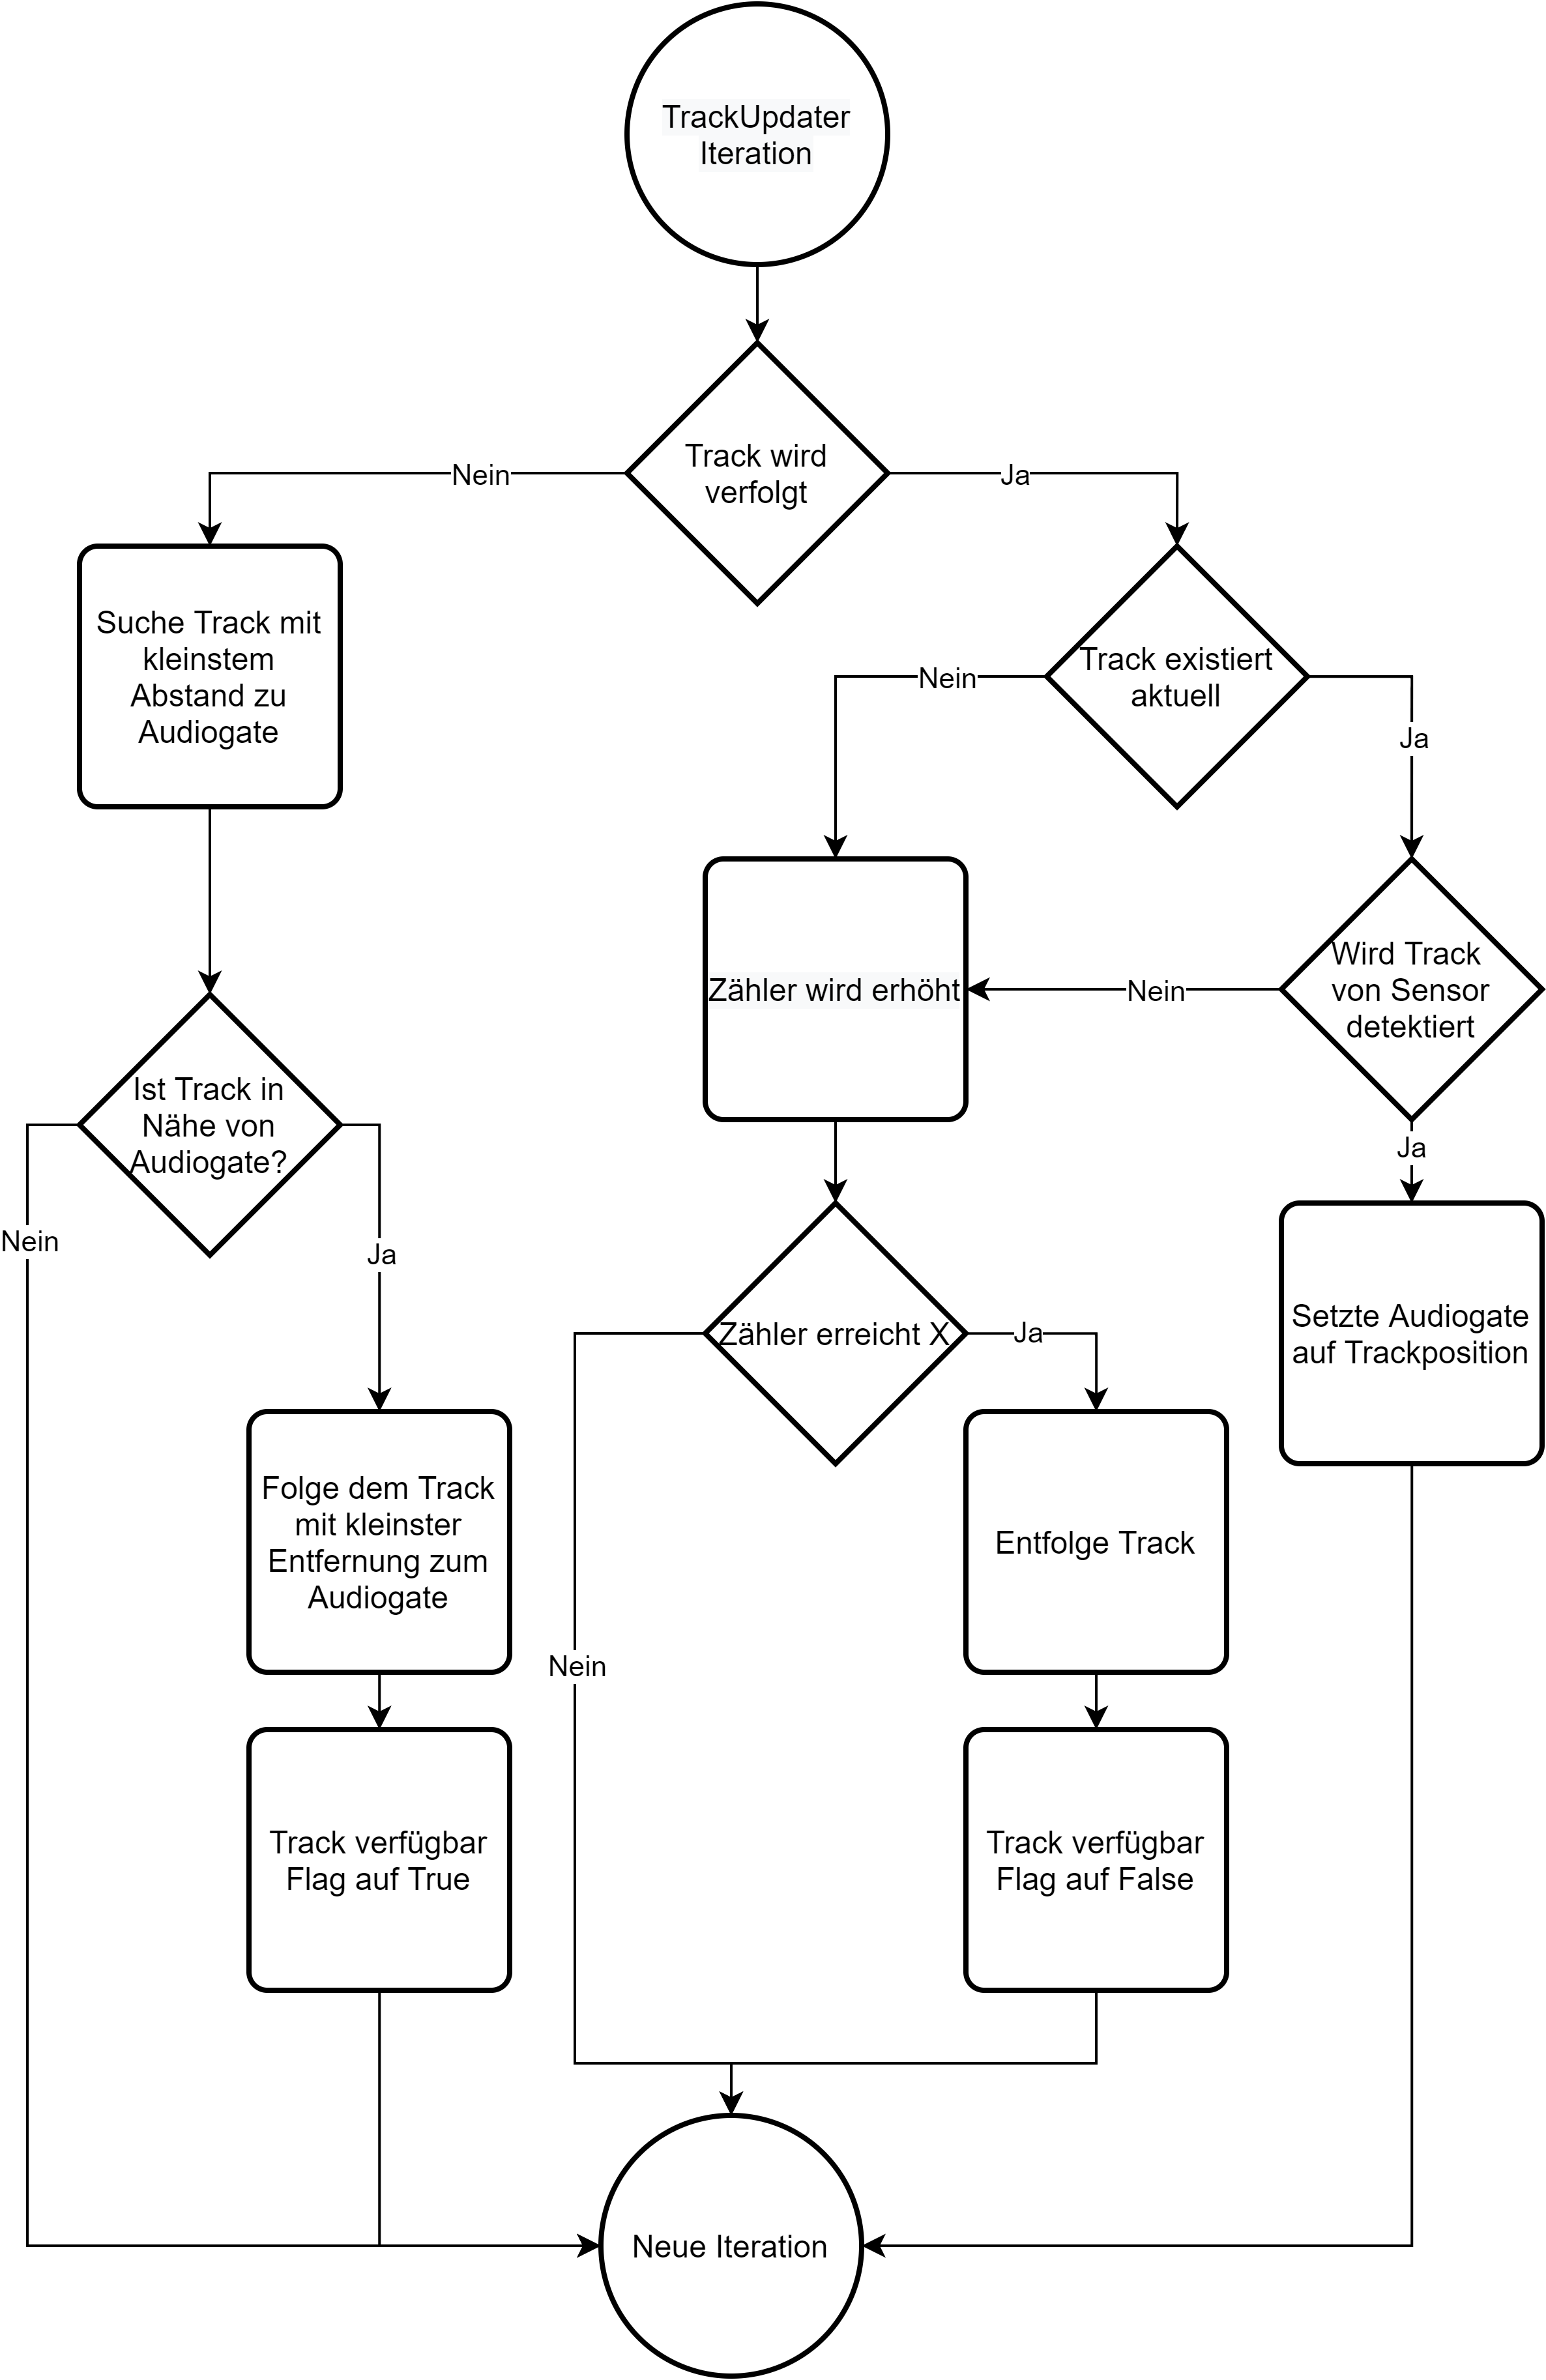
\includegraphics[width=0.65\textwidth]{content/assets/TrackUpdaterSTT.png}
    \caption{Flussdiagramm des Algorithmus des Trackupdaters}
\end{figure}

